\documentclass[12pt]{article}

% Codificación y lenguaje
\usepackage[utf8]{inputenc}
\usepackage[T1]{fontenc}
\usepackage[spanish]{babel}
\usepackage{tikz}
\usetikzlibrary{positioning, arrows.meta}
\usepackage{graphicx} 
\usepackage{tabularx}
\usepackage{hyperref} 

% Márgenes
\usepackage[a4paper, left=2.5cm, right=2.5cm, top=2cm, bottom=2cm]{geometry}

% Gráficos, flotantes y código
\usepackage{graphicx}
\usepackage{caption}
\usepackage{float}
\usepackage{listings}
\usepackage{xcolor}
\usepackage{tikz}
\usepackage{url}


% Encabezados y pies de página
\usepackage{fancyhdr}
\pagestyle{fancy}
\fancyhf{}
\lhead{TP Nº3 - Transformada Rápida de Fourier}
\rhead{UNC-Procesamiento digital de señales}
\cfoot{\thepage}
\setlength{\headheight}{15pt}

% Estilo para código Matlab
\definecolor{codegreen}{rgb}{0,0.6,0}
\definecolor{codegray}{rgb}{0.5,0.5,0.5}
\definecolor{codepurple}{rgb}{0.58,0,0.82}
\definecolor{backcolour}{rgb}{0.95,0.95,0.92}

\lstdefinestyle{mystyle}{
	language=C,
	backgroundcolor=\color{white},
	basicstyle=\scriptsize\ttfamily,           % Tamaño de fuente reducido con tipografía monoespaciada
	keywordstyle=\color[HTML]{0072BD}\bfseries,
	commentstyle=\color[HTML]{008000}\itshape,
	stringstyle=\color[HTML]{A2142F},
	numberstyle=\tiny\color{gray},             % Números de línea discretos
	numbers=left,
	numbersep=6pt,                             % Separación más generosa para claridad
	frame=single,
	rulecolor=\color{black!50},
	breaklines=true,                           % Cortar líneas largas automáticamente
	breakatwhitespace=false,                   % Cortar incluso sin espacios
	breakautoindent=true,                      % Mantener indentación visual
	tabsize=2,
	showspaces=false,
	showstringspaces=false,
	xleftmargin=1.5em,                         % Margen izquierdo para números
	xrightmargin=0.5em,
	aboveskip=1em,                             % Espacio antes del bloque de código
	belowskip=1em,                             % Espacio después del bloque de código
}

\lstdefinestyle{pythonstyle}{
	language=Python,
	backgroundcolor=\color{white},
	basicstyle=\scriptsize\ttfamily,
	keywordstyle=\color[HTML]{0000FF}\bfseries,
	commentstyle=\color[HTML]{008000}\itshape,
	stringstyle=\color[HTML]{A2142F},
	numberstyle=\tiny\color{gray},
	numbers=left,
	numbersep=6pt,
	frame=single,
	rulecolor=\color{black!50},
	breaklines=true,
	breakatwhitespace=false,
	breakautoindent=true,
	tabsize=4,
	showspaces=false,
	showstringspaces=false,
	xleftmargin=1.5em,
	xrightmargin=0.5em,
	aboveskip=1em,
	belowskip=1em
}


% Título y autores
\title{
	
\includegraphics[width=0.45\textwidth]{unc.png} \\[2cm] % Logo
	\textbf{Trabajo Práctico Nº3: Transformada Rápida de Fourier} 
}
    
\author{
	Profesores: \\ Parlanti Gustavo Fernand (Presidente) \\ Molina German Alcides (Vocal)\\ Rossi Robreto Raul (Vocal)
	\\ \\
	Alumnos:\\ Campos \\ Testa \\ Verstraete 
}

\date{Abril de 2026} % Fecha del trabajo

\begin{document}
	
	\maketitle
	
	\begin{abstract}
	
    Realizar un programa aplicativo que sea capaz de implementar la Transformada Rápida de Fourier (FFT) sobre un buffer de memoria de tamaño configurable (512, 1024 y 2048 muestras), cuyos datos son adquiridos a partir del sistema desarrollado en el Laboratorio Nº1, contemplando además las distintas frecuencias de muestreo disponibles (8 kHz, 16 kHz, 24 kHz, 40 kHz y 48 kHz). El sistema permitirá habilitar o deshabilitar la aplicación de la FFT mediante una tecla de la placa de evaluación, funcionando en modo procesamiento o bypass. El resultado de la FFT será transmitido a través del puerto serie (SDU) para su posterior visualización en una PC mediante una herramienta gráfica, donde se representará el espectro de la señal.  

	\end{abstract}\newpage
	
	\tableofcontents \newpage
	
	\section{Introducción}
	
		El análisis espectral de señales constituye una herramienta fundamental dentro del procesamiento digital de señales (DSP), ya que permite representar una señal en el dominio de la frecuencia y extraer información relevante sobre su contenido armónico. En sistemas embebidos, la implementación eficiente de este tipo de análisis resulta clave en aplicaciones como procesamiento de audio, monitoreo de vibraciones, telecomunicaciones y sistemas de diagnóstico.

		En este trabajo práctico se aborda la implementación de la Transformada Rápida de Fourier (FFT) sobre una plataforma basada en el microcontrolador STM32F446RE, continuando con la arquitectura desarrollada en los laboratorios anteriores. El sistema permite adquirir señales analógicas mediante el ADC, procesarlas en tiempo real y analizar su espectro de frecuencias utilizando buffers de distinto tamaño (512, 1024 y 2048 muestras), lo que introduce un compromiso entre resolución espectral y carga computacional.

		Para garantizar el funcionamiento en tiempo real, se mantiene el uso de técnicas eficientes como transferencias mediante DMA en modo circular y procesamiento por bloques, minimizando la intervención del CPU. Asimismo, se emplea la biblioteca CMSIS-DSP, optimizada para arquitecturas ARM Cortex-M, que permite implementar la FFT de manera eficiente en formato de punto fijo.

		El sistema desarrollado permite habilitar o deshabilitar el procesamiento mediante una tecla de usuario (modo FFT o bypass), y transmitir los resultados a través de una interfaz serie hacia una PC, donde se visualiza el espectro de la señal. Esto posibilita analizar el impacto de parámetros clave como la frecuencia de muestreo y el tamaño de la ventana sobre la resolución en frecuencia, la observación de efectos de aliasing asociados al proceso de muestreo y las limitaciones prácticas del sistema.

		De esta manera, el trabajo no solo busca implementar la FFT en un entorno embebido, sino también comprender los compromisos inherentes al análisis espectral en tiempo real, integrando conceptos teóricos con su aplicación práctica sobre hardware real.

		\subsection{Objetivos del proyecto}
		
			\begin{itemize}
			\item Implementar la Transformada Rápida de Fourier (FFT) sobre señales adquiridas en tiempo real utilizando el ADC del microcontrolador STM32F446RE.
			
			\item Procesar buffers de distinto tamaño (512, 1024 y 2048 muestras), analizando el impacto en la resolución espectral y el rendimiento del sistema.
			
			\item Integrar el procesamiento de la FFT dentro de la arquitectura basada en DMA y doble buffering, garantizando operación en tiempo real.
			
			\item Utilizar la biblioteca CMSIS-DSP para la implementación eficiente de la FFT en formato de punto fijo (Q15).
			
			\item Permitir la habilitación o deshabilitación del procesamiento (modo FFT/bypass) mediante una entrada por GPIO.
			
			\item Transmitir los resultados de la FFT a través de una interfaz serie (SDU) para su posterior visualización en una PC.
			
			\item Analizar el espectro de la señal obtenida, evaluando el efecto de la frecuencia de muestreo y el tamaño de la ventana sobre la resolución en frecuencia.
			
			\end{itemize}
			
	\section{Marco teórico}

		\subsection{Análisis espectral de señales}

			El análisis espectral consiste en representar una señal en el dominio de la frecuencia, permitiendo identificar las componentes sinusoidales que la conforman. Mientras que en el dominio temporal se observa la evolución de la señal en el tiempo, el dominio frecuencial permite analizar su contenido armónico, lo cual resulta fundamental en aplicaciones de procesamiento de audio, comunicaciones y sistemas de medición.

			Para señales digitales, este análisis se realiza a partir de muestras discretas en el tiempo, obtenidas mediante un proceso de muestreo. La precisión del análisis espectral depende directamente de parámetros como la frecuencia de muestreo y la cantidad de muestras consideradas.

		\subsection{Transformada Discreta de Fourier (DFT)} 

			La Transformada Discreta de Fourier (DFT) es una herramienta matemática que permite transformar una señal discreta en el tiempo $x[n]$ en su representación en frecuencia $X[k]$. Se define como:

			\[
			X[k] = \sum_{n=0}^{N-1} x[n] \cdot e^{-j 2\pi \frac{k n}{N}}, \quad k = 0,1,2,\dots,N-1
			\]

			donde $N$ es la cantidad de muestras de la señal. Cada valor $X[k]$ representa la contribución de una componente de frecuencia específica dentro de la señal.

			El principal inconveniente de la DFT es su alto costo computacional, ya que requiere del orden de $O(N^2)$ operaciones, lo cual la vuelve poco eficiente para aplicaciones en tiempo real sobre sistemas embebidos.

		\subsection{Transformada Rápida de Fourier (FFT)}

			La Transformada Rápida de Fourier (FFT) es un algoritmo optimizado para calcular la DFT de manera eficiente, reduciendo la complejidad computacional a $O(N \log_2 N)$. Esto la hace viable para implementaciones en tiempo real.

			El algoritmo más común es el de tipo Cooley-Tukey, el cual se basa en dividir recursivamente la DFT en transformadas más pequeñas.

			El procedimiento general consiste en:

			\begin{itemize}
				\item Reordenar las muestras de entrada según el esquema de inversión de bits (bit-reversal).
				\item Dividir el problema en etapas, donde en cada una se combinan pares de muestras mediante operaciones conocidas como \textit{butterflies}.
				\item Aplicar factores de rotación complejos (twiddle factors), definidos como:
			\end{itemize}

			\[
			W_N^k = e^{-j 2\pi \frac{k}{N}}
			\]

			\noindent
			A lo largo de $\log_2 N$ etapas, se obtiene finalmente el espectro completo de la señal.

		\subsection{Resolución espectral y parámetros de análisis}

			La resolución en frecuencia de la FFT está dada por:

			\[
			\Delta f = \frac{f_s}{N}
			\]
		
			donde $f_s$ es la frecuencia de muestreo y $N$ el número de muestras. Esto implica que:

			\begin{itemize} 
				\item A mayor tamaño de ventana ($N$), mayor resolución en frecuencia.
				\item A mayor frecuencia de muestreo, mayor ancho de banda analizado.
			\end{itemize}

			Sin embargo, existe un compromiso entre resolución espectral y tiempo de procesamiento, ya que buffers más grandes implican mayor carga computacional y latencia.

			Además, en implementaciones prácticas pueden aparecer fenómenos como:

			\begin{itemize}
				\item \textbf{Aliasing}: debido a una frecuencia de muestreo insuficiente.
				\item \textbf{Fuga espectral (spectral leakage)}: causada por el truncamiento de la señal en ventanas finitas.
				\item \textbf{Resolución limitada}: cuando las componentes espectrales están muy cercanas entre sí.
			\end{itemize}

		\subsection{Implementación en sistemas embebidos}

			En sistemas embebidos, la FFT se aplica sobre bloques de datos adquiridos en tiempo real. Para ello, es común utilizar buffers circulares y técnicas de doble buffering, permitiendo procesar un bloque mientras el siguiente se está adquiriendo.

			El uso de aritmética en punto fijo, como el formato Q15, permite reducir el uso de memoria, mantener compatibilidad con el esquema de procesamiento implementado en los trabajos previos y emplear rutinas optimizadas de CMSIS-DSP. Si bien el STM32F446RE dispone de unidad de punto flotante de simple precisión, el formato Q15 resulta adecuado para representar señales adquiridas mediante un ADC de 12 bits y realizar procesamiento eficiente sobre bloques de datos.

		\subsection{Biblioteca CMSIS-DSP}

			La biblioteca CMSIS-DSP proporciona funciones optimizadas para procesamiento digital de señales en microcontroladores ARM Cortex-M. Incluye implementaciones eficientes de la FFT tanto en punto flotante como en punto fijo (Q15 y Q31).

			Para el cálculo de la FFT en formato Q15, se utilizan funciones como:

			\begin{itemize}
				\item \texttt{arm\_rfft\_q15}: para señales reales.
				\item \texttt{arm\_cfft\_q15}: para señales complejas.
			\end{itemize}

			Estas funciones requieren la inicialización previa de una estructura de configuración, la cual contiene parámetros como el tamaño de la FFT y los factores de rotación precomputados.

			El flujo típico de implementación es:

			\begin{enumerate}
				\item Conversión de las muestras del ADC al formato Q15.
				\item Inicialización de la estructura de la FFT.
				\item Ejecución de la FFT sobre el buffer de entrada.
				\item Cálculo de la magnitud del espectro (por ejemplo, mediante \texttt{arm\_cmplx\_mag\_q15}).
			\end{enumerate}

			Estas rutinas están altamente optimizadas y aprovechan las instrucciones SIMD del núcleo Cortex-M4, permitiendo una ejecución eficiente en aplicaciones de tiempo real.

			
	\section{Placa de Desarrollo y Herramientas Utilizadas}
		El proyecto fue desarrollado sobre la placa STM32 Nucleo-F446RE, basada en el microcontrolador STM32F446RE, perteneciente a la familia STM32F4 de STMicroelectronics. Esta plataforma integra una arquitectura avanzada ARM Cortex-M4, periféricos orientados a procesamiento de señales, y herramientas de desarrollo que permiten implementar sistemas en tiempo real de forma eficiente.
		
		\begin{figure}[h!]
			\centering
			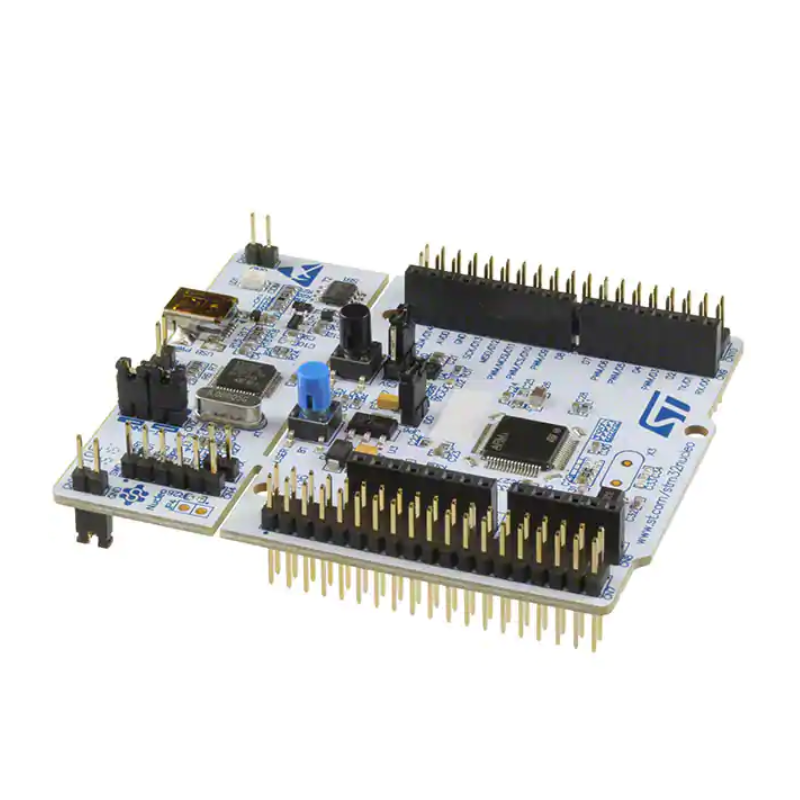
\includegraphics[width=0.7\linewidth]{placa}
			\caption[Placa de desarrollo]{Placa de desarrollo}
			\label{fig:placa}
		\end{figure}
	
		\subsection{Microcontrolador STM32F446RE}

			El STM32F446RE es un microcontrolador de 32 bits basado en el núcleo ARM Cortex-M4, optimizado para procesamiento digital con soporte de instrucciones DSP y unidad de punto flotante opcional (FPU simple precisión). Sus principales características relevantes al proyecto son:

			\begin{itemize}
				\item Frecuencia de operación: hasta 180 MHz
				
				\item Memoria Flash: 512 KB
				
				\item RAM: 128 KB
				
				\item Tensión de operación: 1.8 V a 3.6 V
				
				\item Paquete: LQFP64 (compatible con la Nucleo-F446RE)
			\end{itemize}
	
		\subsection{Periféricos clave utilizados}

			\subsubsection{ADC (Analog-to-Digital Converter)}
			
			\subsubsection{DAC (Digital-to-Analog Converter)}
			
			\subsubsection{DMA (Direct Memory Access)}
			
			\subsubsection{TIM (Timers)}
			
			\subsubsection{GPIO – General Purpose Input/Output}
			
			\subsubsection{Herramientas de desarrollo}

	%--------------------------------------------------------%

	\section{Diseño del programa}

	%--------------------------------------------------------%

	\section{Programa principal}

		\subsection{Configuración de periféricos}
		
			\subsubsection{Configuración del ADC}
			
			\subsubsection{Configuración del DAC}
			
			\subsubsection{Configuración del temporizador}
			
			\subsubsection{Configuración del DMA}
			
			\subsubsection{Configuración de GPIO}
			
			\subsubsection{Inicialización de los filtros digitales}
			
			\subsubsection{Ejecución en tiempo real}
		
	\section{Resultados experimentales}

	%--------------------------------------------------------%
	
	\section{Conclusiones}

	%--------------------------------------------------------%

\end{document}
